



\chapter{Boundaries}\label{chap:boundaries}

Now will be discussed are the multi-structures that constitute the boundaries of other multi-structures. There will be the endpoints of multi-paths, the boundaries of multi-surfaces, and the surfaces of multi-volumes. Throughout the discussion the symbol ``\(\nabla\)", referred to as a ``nabla", will see frequent use. One possible interpretation of \(\nabla\) is:

\[\nabla = \text{``the inwards oriented surface of reality"}\]

By ``inwards oriented surface of reality", reality is in ``front" of \(\nabla\), and ``un-reality" is behind \(\nabla\). \(\nabla\) {\bf is not an actual 2D surface}, but this interpretation is useful regardless.



\section{Point totals}

Given a multi-point \(\rho\), the total sum of the weights of all of the points that comprise \(\rho\) is denoted by:

\[\int \rho\]

The elongated \(S\), \(\int\), literally stands for sum.

If \(\rho = w_1 P_1 + w_2 P_2 + ... + w_N P_N\) where \(P_1\), \(P_2\), ..., \(P_N\) are single points, then
\[\int \rho = \int (w_1 P_1 + w_2 P_2 + ... + w_N P_N) = w_1 + w_2 + ... + w_N\]

\begin{center} 
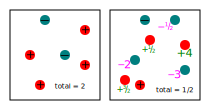
\includegraphics[width = 0.5\textwidth]{Point_totals/multi-point_sums}
\end{center}


\subsection{Scanning for equivalence}

In chapter \ref{chap:multi-structures}, descriptions of what it means for two multi-structures to be equivalent were briefly given. 

\begin{itemize}
\item Two multi-points \(\rho_1\) and \(\rho_2\) are equivalent if and only if the collections of constituent points are equivalent with identical weights. 
\item Two multi-paths \(\mathbf{J}_1\) and \(\mathbf{J}_2\) are equivalent if and only if the networks of oriented paths are equivalent, regardless of how the network is broken up into individual oriented paths. Within the same multi-path, path sections with opposite orientations cancel each other out. 
\item Two multi-surfaces \(\mathbf{F}_1\) and \(\mathbf{F}_2\) are equivalent if and only if the networks of oriented surfaces are equivalent, regardless of how the network is broken up into individual oriented surfaces. Within the same multi-surface, surface sections with opposite orientations cancel each other out. 
\item Two multi-volumes \(U_1\) and \(U_2\) are equivalent if and only if at every position \(\mathbf{q}\), the net number of volumes from \(U_1\) that contain \(\mathbf{q}\) is equal to the net number of volumes from \(U_2\) that contain \(\mathbf{q}\). Negative volumes subtract from the number of volumes that contain \(\mathbf{q}\). 
\end{itemize}

The equivalence of two multi-structures can alternately be determined by moving around a small ``scanning window" and then comparing the total intersection point weights found within the scanning window. If the numbers of detected intersection points are equivalent between the two multi-structures no matter the choice of scanning window, then the two multi-structures must be equivalent. This is elaborated in more detail below

\subsubsection{Scanning multi-points}

Two multi-points can be determined to be equal by ``scanning" for differences between the two multi-points using a small volume ``scanning window". Let \(\rho\) denote an arbitrary multi-point. If \(U\) is a tiny single volume, then \(\int (\rho \cdot U)\) is the number of points (weighted accordingly) from \(\rho\) that are found within the tiny ``scanning window" \(U\). By moving the scanning window \(U\) around as well as adjusting the size, and then computing \(\int (\rho \cdot U)\), the constituent points from \(\rho\) can effectively be ``felt" for, and differences between the multi-points identified.  

\begin{thm}\label{thm:scanning_points}
If \(\rho_1\) and \(\rho_2\) are equivalent multi-points: \(\rho_1 = \rho_2\), then for any choice of multi-volume \(U\), 
\[\int (\rho_1 \cdot U) = \int (\rho_2 \cdot U)\]
Conversely, if \(\rho_1\) and \(\rho_2\) are multi-points, but it is instead known that for any choice of multi-volume \(U\) that 
\(\int (\rho_1 \cdot U) = \int (\rho_2 \cdot U)\), then \(\rho_1\) and \(\rho_2\) are in fact equivalent:
\[\rho_1 = \rho_2\]  
\end{thm}
\textbf{Proof:}

If \(\rho_1 = \rho_2\), then it is fairly obvious from the equivalence of \(\rho_1\) and \(\rho_2\) that \(\int (\rho_1 \cdot U) = \int (\rho_2 \cdot U)\) for all choices of multi-volume \(U\). 

\begin{tabular}{cc}
\parbox{0.5\textwidth}{
With respect to the converse, assume that \(\rho_1 \neq \rho_2\). Since \(\rho_1 \neq \rho_2\), there must exist some point in \(\rho_1\) that has a different weight, possibly \(0\), in \(\rho_2\). There will then exist some small scanning window \(U\) that wraps the point in question, and captures a different amount of point weight in \(\rho_1\) than in \(\rho_2\).

In the image on the right, the difference between \(\rho_1\) and \(\rho_2\) is targeted by the scanning window \(U\). A different amount of point weight is captured by \(U\) for \(\rho_1\) and \(\rho_2\), so \(\int (\rho_1 \cdot U) \neq \int (\rho_2 \cdot U)\).
} & \parbox{0.5\textwidth}{
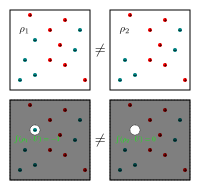
\includegraphics[width = 0.5\textwidth]{Point_totals/scanning_points_using_volumes}
}
\end{tabular}

\(\Box\)

\subsubsection{Scanning multi-paths}

Two multi-paths can be determined to be equal by ``scanning" for differences between the two multi-paths using a small surface ``scanning window". Let \(\mathbf{J}\) denote an arbitrary multi-path. If \(\mathbf{F}\) is a tiny single surface, then \(\int (\mathbf{J} \bullet \mathbf{F})\) is the number of intersection points (weighted accordingly) resulting from \(\mathbf{J}\) intersecting the tiny ``scanning window" \(\mathbf{F}\). By moving the scanning window \(\mathbf{F}\) around as well as adjusting the size, and then computing \(\int (\mathbf{J} \bullet \mathbf{F})\), the constituent paths from \(\mathbf{J}\) can effectively be ``felt" for, and differences between the multi-paths identified.  

\begin{thm}\label{thm:scanning_paths}
If \(\mathbf{J}_1\) and \(\mathbf{J}_2\) are equivalent multi-paths: \(\mathbf{J}_1 = \mathbf{J}_2\), then for any choice of multi-surface \(\mathbf{F}\), 
\[\int (\mathbf{J}_1 \bullet \mathbf{F}) = \int (\mathbf{J}_2 \bullet \mathbf{F})\]
Conversely, if \(\mathbf{J}_1\) and \(\mathbf{J}_2\) are multi-paths, but it is instead known that for any choice of multi-surface \(\mathbf{F}\) that 
\(\int (\mathbf{J}_1 \bullet \mathbf{F}) = \int (\mathbf{J}_2 \bullet \mathbf{F})\), then \(\mathbf{J}_1\) and \(\mathbf{J}_2\) are in fact equivalent:
\[\mathbf{J}_1 = \mathbf{J}_2\]  
\end{thm}
\textbf{Proof:}

If \(\mathbf{J}_1 = \mathbf{J}_2\), then it is fairly obvious from the equivalence of \(\mathbf{J}_1\) and \(\mathbf{J}_2\) that \(\int (\mathbf{J}_1 \bullet \mathbf{F}) = \int (\mathbf{J}_2  \bullet \mathbf{F})\) for all choices of multi-surface \(\mathbf{F}\). 

\vspace{5mm}

\begin{tabular}{cc}
\parbox{0.5\textwidth}{
With respect to the converse, assume that \(\mathbf{J}_1 \neq \mathbf{J}_2\). Since \(\mathbf{J}_1 \neq \mathbf{J}_2\), there must exist some path in \(\mathbf{J}_1\) that has a different weight, possibly \(0\), or a different shape in \(\mathbf{J}_2\). There will then exist some small scanning window \(\mathbf{F}\) that intersects the path in question, and records a different amount of intersection point weight from \(\mathbf{J}_1\) than from \(\mathbf{J}_2\).

In the image on the right, the difference between \(\mathbf{J}_1\) and \(\mathbf{J}_2\) is targeted by the scanning window \(\mathbf{F}\). A different amount of intersection point weight is captured by \(\mathbf{F}\) for \(\mathbf{J}_1\) and \(\mathbf{J}_2\), so \(\int (\mathbf{J}_1 \bullet \mathbf{F}) \neq \int (\mathbf{J}_2 \bullet \mathbf{F})\).
} & \parbox{0.5\textwidth}{
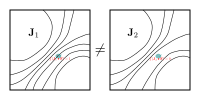
\includegraphics[width = 0.5\textwidth]{Point_totals/scanning_paths_using_surfaces}
}
\end{tabular}

\(\Box\)

\subsubsection{Scanning multi-surfaces}

Two multi-surfaces can be determined to be equal by ``scanning" for differences between the two multi-surfaces using a small path ``scanning window". Let \(\mathbf{F}\) denote an arbitrary multi-surface. If \(\mathbf{J}\) is a tiny single path, then \(\int (\mathbf{F} \bullet \mathbf{J})\) is the number of intersection points (weighted accordingly) resulting from \(\mathbf{F}\) intersecting the tiny ``scanning window" \(\mathbf{J}\). By moving the scanning window \(\mathbf{J}\) around as well as adjusting the length, and then computing \(\int (\mathbf{F} \bullet \mathbf{J})\), the constituent surfaces from \(\mathbf{F}\) can effectively be ``felt" for, and differences between the multi-surfaces identified.  

\begin{thm}\label{thm:scanning_surfaces}
If \(\mathbf{F}_1\) and \(\mathbf{F}_2\) are equivalent multi-surfaces: \(\mathbf{F}_1 = \mathbf{F}_2\), then for any choice of multi-path \(\mathbf{J}\), 
\[\int (\mathbf{F}_1 \bullet \mathbf{J}) = \int (\mathbf{F}_2 \bullet \mathbf{J})\]
Conversely, if \(\mathbf{F}_1\) and \(\mathbf{F}_2\) are multi-surfaces, but it is instead known that for any choice of multi-path \(\mathbf{J}\) that 
\(\int (\mathbf{F}_1 \bullet \mathbf{J}) = \int (\mathbf{F}_2 \bullet \mathbf{J})\), then \(\mathbf{F}_1\) and \(\mathbf{F}_2\) are in fact equivalent:
\[\mathbf{F}_1 = \mathbf{F}_2\]  
\end{thm}
\textbf{Proof:}

If \(\mathbf{F}_1 = \mathbf{F}_2\), then it is fairly obvious from the equivalence of \(\mathbf{F}_1\) and \(\mathbf{F}_2\) that \(\int (\mathbf{F}_1 \bullet \mathbf{J}) = \int (\mathbf{F}_2  \bullet \mathbf{J})\) for all choices of multi-path \(\mathbf{J}\). 

\vspace{5mm}

\begin{tabular}{cc}
\parbox{0.5\textwidth}{
With respect to the converse, assume that \(\mathbf{F}_1 \neq \mathbf{F}_2\). Since \(\mathbf{F}_1 \neq \mathbf{F}_2\), there must exist some surface in \(\mathbf{F}_1\) that has a different weight, possibly \(0\), or a different shape in \(\mathbf{F}_2\). There will then exist some small scanning window \(\mathbf{J}\) that intersects the surface in question, and records a different amount of intersection point weight from \(\mathbf{F}_1\) than from \(\mathbf{F}_2\).

In the image on the right, the difference between \(\mathbf{F}_1\) and \(\mathbf{F}_2\) is targeted by the scanning window \(\mathbf{J}\). A different amount of intersection point weight is captured by \(\mathbf{J}\) for \(\mathbf{F}_1\) and \(\mathbf{F}_2\), so \(\int (\mathbf{F}_1 \bullet \mathbf{J}) \neq \int (\mathbf{F}_2 \bullet \mathbf{J})\).
} & \parbox{0.5\textwidth}{
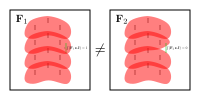
\includegraphics[width = 0.5\textwidth]{Point_totals/scanning_surfaces_using_paths}
}
\end{tabular}

\(\Box\)

\subsubsection{Scanning multi-volumes}

Two multi-volumes can be determined to be equal by ``scanning" for differences between the two multi-volumes using ``point probes". Let \(U\) denote an arbitrary multi-volume. If \(\rho\) is a single point, then \(\int (U \cdot \rho)\) is the number of volumes (weighted accordingly) from \(U\) that contain the probe \(\rho\). By moving the probe \(\rho\) around, and then computing \(\int (U \cdot \rho)\), the constituent volumes from \(U\) can effectively be ``felt" for, and differences between the multi-volumes identified.  

\begin{thm}\label{thm:scanning_volumes}
If \(U_1\) and \(U_2\) are equivalent multi-volumes: \(U_1 = U_2\), then for any choice of multi-point \(\rho\), 
\[\int (U_1 \cdot \rho) = \int (U_2 \cdot \rho)\]
Conversely, if \(U_1\) and \(U_2\) are multi-volumes, but it is instead known that for any choice of multi-point \(\rho\) that 
\(\int (U_1 \cdot \rho) = \int (U_2 \cdot \rho)\), then \(U_1\) and \(U_2\) are in fact equivalent:
\[U_1 = U_2\]  
\end{thm}
\textbf{Proof:}

If \(U_1 = U_2\), then it is fairly obvious from the equivalence of \(U_1\) and \(U_2\) that \(\int (U_1 \cdot \rho) = \int (U_2 \cdot \rho)\) for all choices of multi-point \(\rho\). 

\vspace{5mm}

\begin{tabular}{cc}
\parbox{0.5\textwidth}{
With respect to the converse, assume that \(U_1 \neq U_2\). Since \(U_1 \neq U_2\), there must exist some volume in \(U_1\) that has a different weight, possibly \(0\), or a different shape in \(U_2\). There will then exist some point probe \(\rho\) that targets the difference in question, and records a different amount of volumes in \(U_1\) than in \(U_2\).

In the image on the right, the difference between \(U_1\) and \(U_2\) is targeted by the point probe \(\rho\). A different amount of volumes is recorded by \(\rho\) for \(U_1\) and \(U_2\), so \(\int (U_1 \cdot \rho) \neq \int (U_2 \cdot \rho)\).
} & \parbox{0.5\textwidth}{
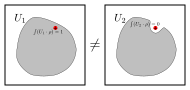
\includegraphics[width = 0.5\textwidth]{Point_totals/scanning_volumes_using_points}
}
\end{tabular}

\(\Box\)





\section{Path endpoints}

Given a multi-path \(\mathbf{J}\), the ``endpoints" of \(\mathbf{J}\) is a multi-point that is denoted by:

\[\nabla \bullet \mathbf{J}\]

Given an oriented path \(C\), let \(P_0\) be the starting point of \(C\), and let \(P_1\) be the finishing point of \(C\). The multi-point that is the endpoints of \(C\) consists of \(P_0\) with a weight of \(+1\) and \(P_1\) with a weight of \(-1\):

\[\nabla \bullet C = P_0 - P_1\]

\begin{center}
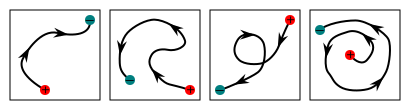
\includegraphics[width = \textwidth]{Boundaries/Path_endpoints/path_endpoint_examples}
\end{center}

The endpoints of a multi-path is the sum of the endpoints of all of the constituent paths:
\[\nabla \bullet (w_1 C_1 + w_2 C_2 + ... + w_N C_N)
= w_1(\nabla \bullet C_1) + w_2(\nabla \bullet C_2) + ... + w_N(\nabla \bullet C_N)\]

\begin{center}
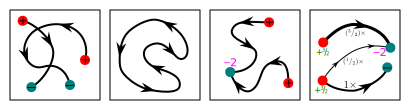
\includegraphics[width = \textwidth]{Boundaries/Path_endpoints/path_endpoint_examples_2}
\end{center}


\begin{thm}
It should be noted that a closed loop has a net endpoint of \(0\). If multi-path \(\mathbf{J}\) consists of only closed loops, then \(\nabla \bullet \mathbf{J} = 0\). 
\end{thm}

It has already been established that paths are not allowed to extend to infinity, hence every starting point must be paired with a finishing point. Starting points have weights of \(+1\), while finishing points have weights of \(-1\). This means that for an arbitrary multi-path \(\mathbf{J}\), that the sum of all of the endpoint weights is \(0\): 
\begin{thm}
For any multi-path \(\mathbf{J}\),
\[\int (\nabla \bullet \mathbf{J}) = 0\] 
\end{thm}

\begin{tabular}{cc}
\parbox{0.5\textwidth}{
A logical question is why the notation \(\nabla \bullet \mathbf{J}\) is used to denote the endpoints of multi-path \(\mathbf{J}\). The notation \(\mathbf{F} \bullet \mathbf{J}\) denotes the intersection of multi-path \(\mathbf{J}\) with multi-surface \(\mathbf{F}\) in the preferred direction. With \(\nabla\) denoting the inwards oriented surface of reality, \(\nabla \bullet \mathbf{J}\) consists of points where \(\mathbf{J}\) enters reality with a weight of \(+1\), and leaves reality with a weight of \(-1\). This is illustrated on the right.
} & \parbox{0.4\textwidth}{
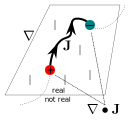
\includegraphics[width = 0.4\textwidth]{Boundaries/Path_endpoints/path_surface_intersections_and_path_endpoints}
}
\end{tabular}




\section{Surface boundaries}

Given a multi-surface \(\mathbf{F}\), the ``boundaries" of \(\mathbf{F}\) is a multi-path that is denoted by: 

\[\nabla \times \mathbf{F}\]

Given an oriented surface \(\sigma\), the boundary of \(\sigma\) is its {\bf counterclockwise} oriented boundary. The counterclockwise orientation is the orientation that traverses the boundary in a counterclockwise direction when the front of the surface is visible. 

More exactly, the counterclockwise orientation is determined as follows. Position your view point so that the front of \(\sigma\) is visible. When \(\sigma\) is on your right, the boundary is oriented towards you. This is demonstrated in the rightmost example below where the boundary circles the hole in a clockwise direction.

\begin{center}
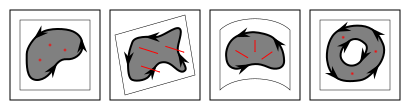
\includegraphics[width = \textwidth]{Boundaries/Surface_boundaries/surface_boundary_examples}
\end{center}

The counterclockwise boundary of a multi-surface is the sum of the boundaries of all of the constituent surfaces:
\[\nabla \times (w_1 \sigma_1 + w_2 \sigma_2 + ... + w_N \sigma_N)
= w_1(\nabla \times \sigma_1) + w_2(\nabla \times \sigma_2) + ... + w_N(\nabla \times \sigma_N)\]

\begin{center}
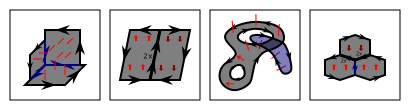
\includegraphics[width = \textwidth]{Boundaries/Surface_boundaries/surface_boundary_examples_2}
\end{center}

\begin{thm}
It should be noted that a closed surface (a bubble) has no boundaries. If multi-surface \(\mathbf{F}\) consists of only closed surfaces (bubbles), then \(\nabla \times \mathbf{F} = 0\). 
\end{thm}

The boundaries of surfaces do not abruptly end, and must be closed loops. The counterclockwise boundaries do not have end points. 
\begin{thm}
For any multi-surface \(\mathbf{F}\), 
\[\nabla \bullet (\nabla \times \mathbf{F}) = 0\]
\end{thm}

\begin{tabular}{cc}
\parbox{0.5\textwidth}{
A logical question is why the notation \(\nabla \times \mathbf{F}\) is used to denote the counterclockwise boundary of multi-surface \(\mathbf{F}\). The notation \(\mathbf{G} \times \mathbf{F}\) denotes the intersection of multi-surface \(\mathbf{G}\) with multi-surface \(\mathbf{F}\), with \(\mathbf{F}\) as the \(2^\text{nd}\) surface. With \(\nabla\) denoting the inwards oriented surface of reality, \(\nabla \times \mathbf{F}\) consists of the path where \(\mathbf{F}\) slices into and out of reality. This is illustrated on the right.
} & \parbox{0.5\textwidth}{
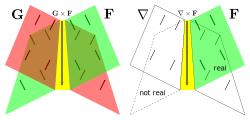
\includegraphics[width = 0.5\textwidth]{Boundaries/Surface_boundaries/right_hand_rule_for_boundaries}
}
\end{tabular}




\section{Volume surfaces}

Given a multi-volume \(U\), the ``surfaces" of \(U\) is a multi-surface that is denoted by: 

\[\nabla U\]

Given a volume \(\Omega\), the surface of \(\Omega\) is {\bf inwards-oriented}. 

\begin{center}
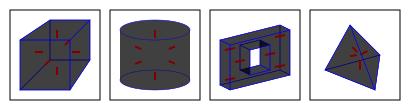
\includegraphics[width = \textwidth]{Boundaries/Volume_inwards_oriented_surfaces/volume_surface_examples}
\end{center}

The inwards oriented surface of a multi-volume is the sum of the inwards oriented surfaces of all of the constituent volumes:
\[\nabla (w_1 \Omega_1 + w_2 \Omega_2 + ... + w_N \Omega_N)
= w_1(\nabla \Omega_1) + w_2(\nabla \Omega_2) + ... + w_N(\nabla \Omega_N)\]

In the examples depicted below, the ``inwards oriented surfaces" of volumes that have a negative weight are in fact oriented outwards.

\begin{center}
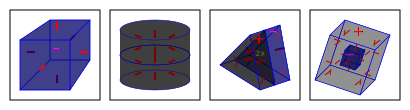
\includegraphics[width = \textwidth]{Boundaries/Volume_inwards_oriented_surfaces/volume_surface_examples_2}
\end{center}

The surfaces of volumes are bubbles that have no boundaries. 
\begin{thm}
For any multi-volume \(U\), 
\[\nabla \times (\nabla U) = 0\]
\end{thm} 

\begin{tabular}{cc}
\parbox{0.5\textwidth}{
A logical question is why the notation \(\nabla U\) is used to denote the inwards oriented surface of multi-volume \(U\). The notation \(\mathbf{F} U\) denotes the intersection of multi-volume \(U\) with multi-surface \(\mathbf{F}\). With \(\nabla\) denoting the inwards oriented surface of reality, \(\nabla U\) consists of the surface where \(U\) pushes into and out of reality. The surface is inwards oriented since \(\nabla\) is inwards oriented. This is illustrated on the right.
} & \parbox{0.3\textwidth}{
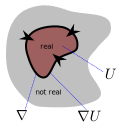
\includegraphics[width = 0.3\textwidth]{Boundaries/Volume_inwards_oriented_surfaces/surface_volume_intersections_and_volume_surfaces}
}
\end{tabular}



\section{Summary}

A summary of the notations used for the different boundaries is given below. In addition, we have observed that the boundaries have no boundaries themselves.

\begin{center}
\begin{tabular}{|c||c|c|c|}
\hline
multi-structure & boundary & orientation & no boundary of the boundary property \\
\hline
\hline
point \(\rho\) \red{\{0\}} &
N/A &
N/A & 
N/A \\ 
\hline 
path \(\mathbf{J}\) \red{\{1\}} & 
point \(\nabla \bullet \mathbf{J}\) \red{\{0\}} & 
positive start, negative end &
\(\int (\nabla \bullet \mathbf{J}) = 0\) \\
\hline
surface \(\mathbf{F}\) \red{\{2\}} & 
path \(\nabla \times \mathbf{F}\) \red{\{1\}} & 
counterclockwise &
\(\nabla \bullet (\nabla \times \mathbf{F}) = 0\) \\
\hline
volume \(U\) \red{\{3\}} & 
surface \(\nabla U\) \red{\{2\}} & 
inwards-oriented & 
\(\nabla \times (\nabla U) = 0\) \\
\hline
\end{tabular}
\end{center}

In \red{red} is indicated the ``dimensionality" of the multi-structure. Points have \(0\) dimensions; paths have \(1\) dimension; surfaces have \(2\) dimensions; and volumes have \(3\) dimensions. The number of dimensions of the boundary is the number of dimensions minus \(1\). When the resultant number of dimensions is less than \(0\), the boundary does not exist.


